\documentclass[10pt,twocolumn,letterpaper]{article}
\usepackage[english]{babel}
\usepackage{cvpr}
\usepackage{times}
\usepackage{epsfig}
\usepackage{graphicx}
\graphicspath{{images/}}
\usepackage{amsmath}
\usepackage{amssymb}
\usepackage{caption}
\usepackage[breaklinks=true,bookmarks=false]{hyperref}

\cvprfinalcopy

\def\httilde{\mbox{\tt\raisebox{-.5ex}{\symbol{126}}}}

\title{\LARGE FormulaTour}

\author{Gianluca Capozzi\\
	"La Sapienza" University of Rome\\
	{\tt\small capozzi.1693255@studenti.uniroma1.it}
	\and
	Marco Costa\\
	"La Sapienza" University of Rome\\
	{\tt\small costa.1691388@studenti.uniroma1.it}
}


\begin{document}
\twocolumn[{%
	\renewcommand\twocolumn[1][]{#1}
	\maketitle
	\begin{center}
		\centering
		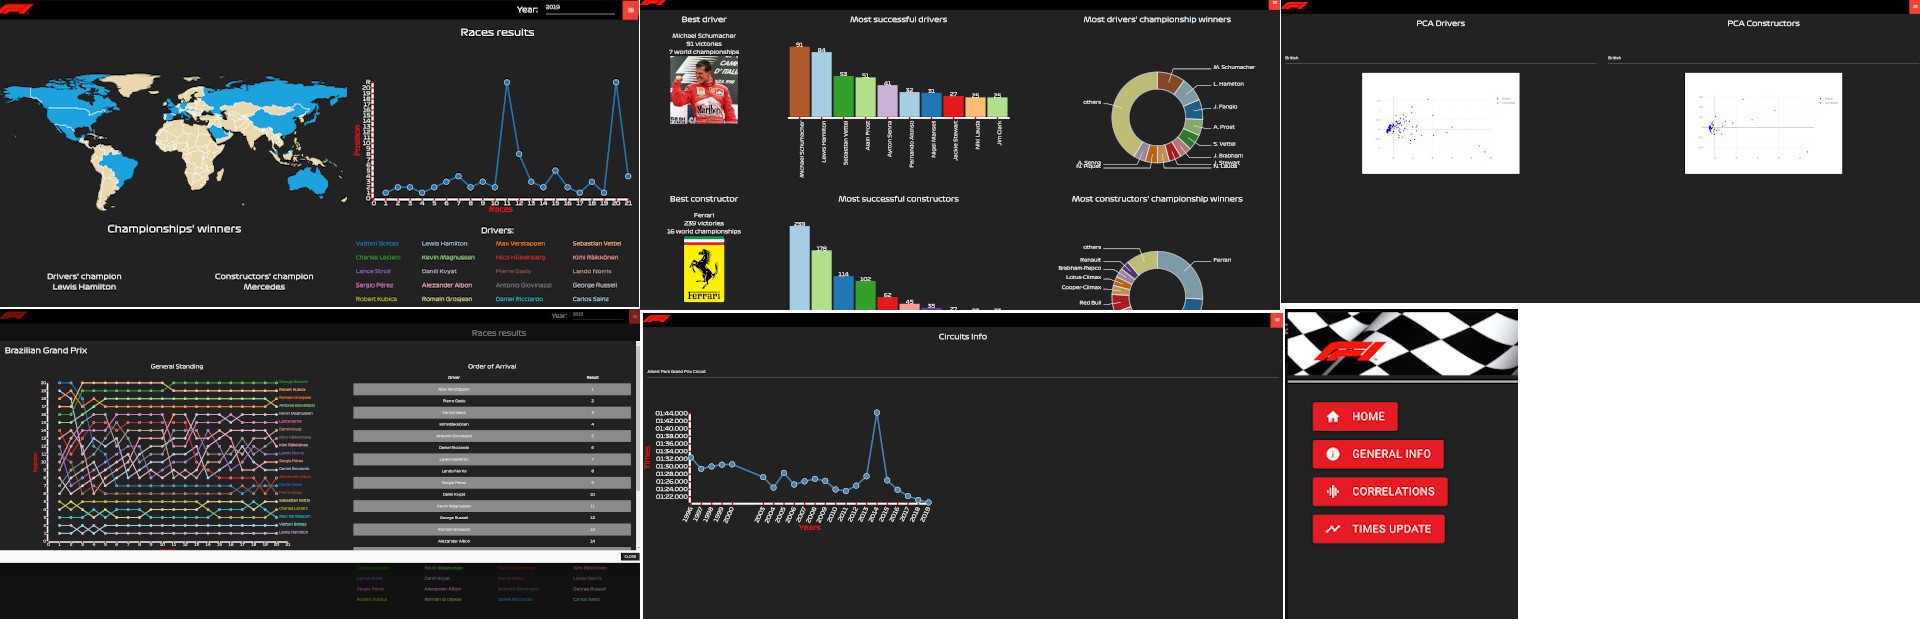
\includegraphics[width=\textwidth]{allViews}
		\captionof{figure}{Framework Views}
	\end{center}
}]

\begin{abstract}

\end{abstract}

\section{Introduction}
Formula 1 has a very long history, as it has reached the $70^{th}$ season. During all these years many drivers and constructors took part to the races, which took
place in different circuits located in different countries. This means that it is very difficult to navigate this history, since it is characterized by many components,
each related to the other. The goal of this project is to provide a way to navigate the history of the Formula 1 by highlighting each component and their relations.
Our framework is divided into four main views each of which contains multiple sub-views. An initial view summarizes the races of the selected season by showing
the countries and the exact location of the circuit in which they took place. A general view summarizes the most important results achieved by the drivers and the
constructors during the Formula 1 history. A correlation view that shows if it exists a correlation between nationalities and number of victories/podiums. The last
view is a times update views that summarizes the evolution of the lap times on a selected circuit during the years. So, our project is composed by:
\begin{itemize}
	\item A visual analytics framework that supports the examination and exploration of Formula 1 history;
	\item A visual representation of the features selected by the users.
\end{itemize}
The project is a web application and it is developed using the d3.js \cite{D3} library and the python3 language for performing PCA.

\section{Related works}
There are other frameworks that show the evolution of Formula 1 through its different elements, so races, drivers and constructors. An example is
\href{https://f1.bitmetric.nl/formula.html}{The history of Formula 1} framework, based on the same dataset used for this project. The main difference is that in that project
there is not a division of the races with respect to the years and also the user is not able to locate geographically the position of the circuits. 

\section{Dataset}
The dataset used for this project is obtained from the Ergast Developer API \cite{Dataset} in .csv format. It is composed by 13 tables: circuits,
constructorResults, constructorStandings, constructors, driverStandings, drivers, lapTimes, pitStops, qualifying, races, results, seasons and status. The tables considered
for this project are:
\begin{itemize}
	\item races: a table that contains informations about each race, as the year and the date in which it was played, the circuitId (which identifies the circuit in which it took place), the name of the Grand Prix (such as Italian Grand Prix) and so on;
	\item circuits: a table that contains informations about each circuit, such as the name of the circuit, its coordinates, the country and so on;
	\item drivers: a table that contains informations about each driver, such as his name and surname, his date of birth, his nationality and so on;
	\item results; a table that, for each race and driver who took part in that race, shows the result of that driver in that race and other infos;
	\item driverStandings: a table that, for each race and driver who took part in that race, shows the driver's point into the drivers' standing after the conclusion of that
	race;
	\item qualifying: a table that, for each race and driver who took part in that race, shows the results that the given driver achieves during the qualifying for that race;
	\item constructors;
	\item constructorStandings. 
\end{itemize}
The .csv files are manipulated using both d3.js and python. Some of the queries performed over the dataset needs the interaction of the user, while others are performed
without parameters chosen by the users.

\section{Visualization}
The visualization is composed by 4 main views, accessible from a simple side menu. Each of these views provides some processed information about the dataset.
\begin{center}
	\centering
	
\includegraphics[width=0.3\columnwidth]{menu}
	\captionof{figure}{Menu}
\end{center}

\subsection{Home view}
\begin{center}
	\centering
	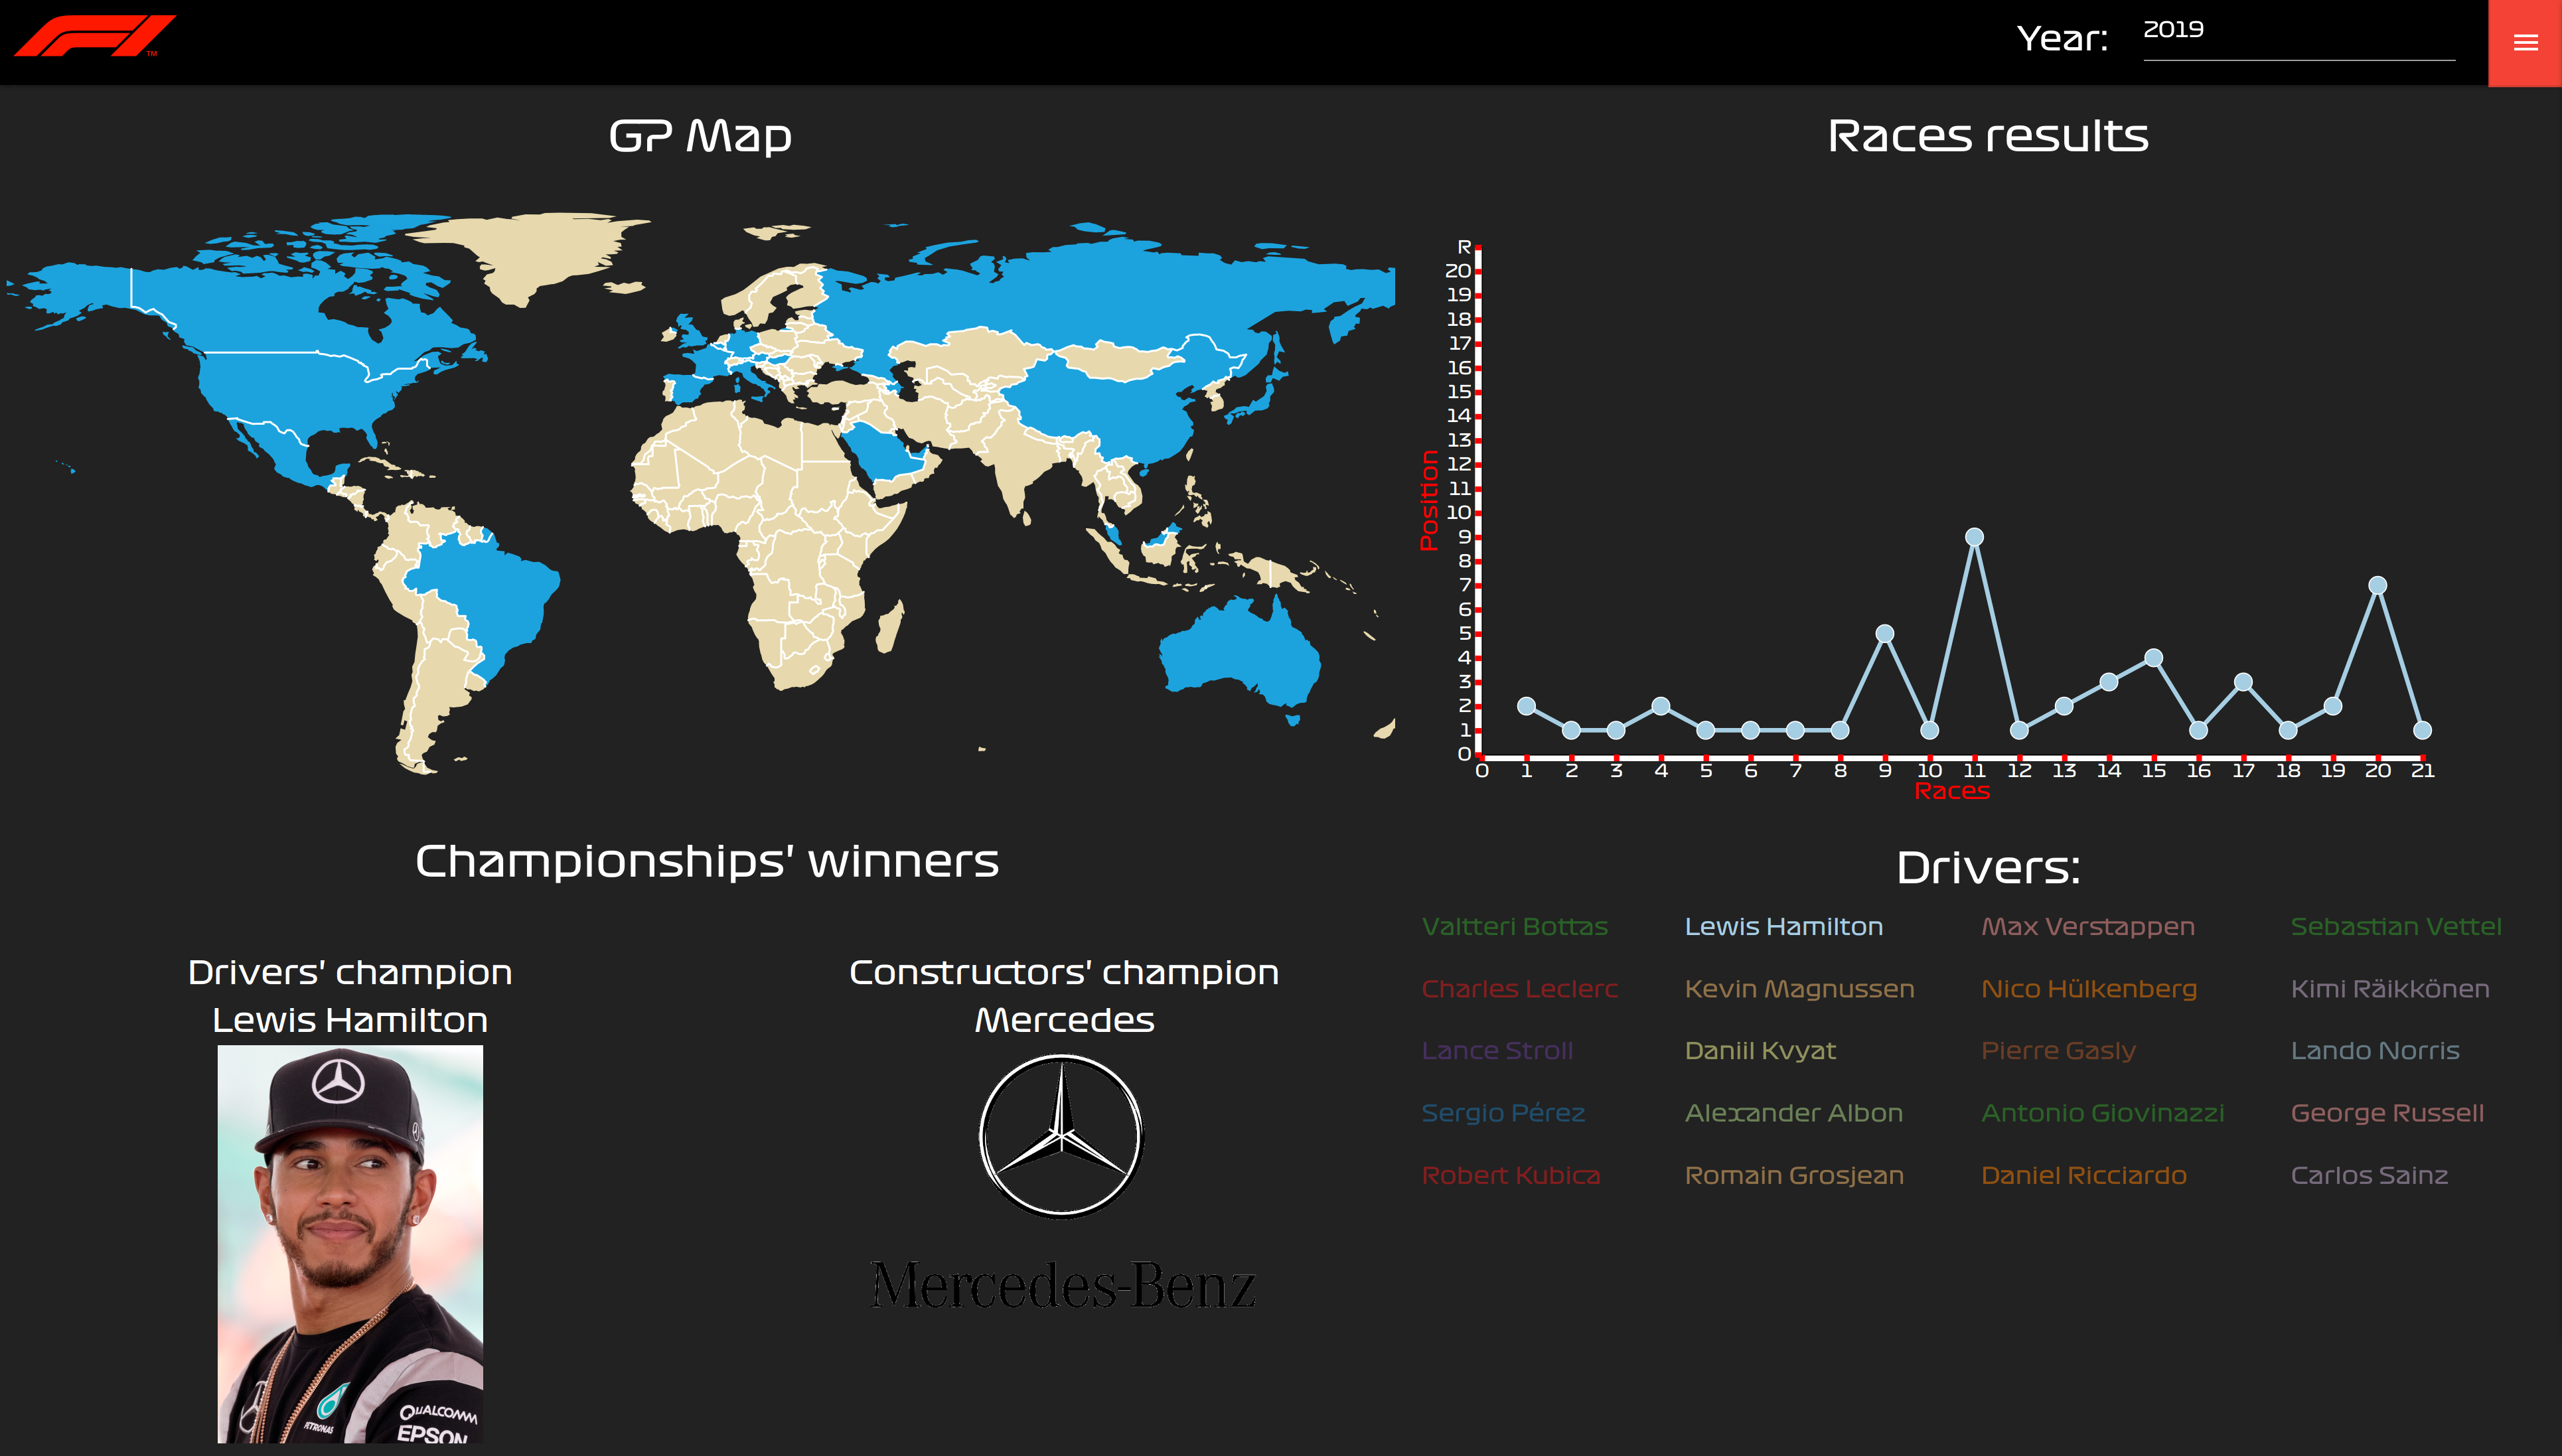
\includegraphics[width=\columnwidth]{home}
	\captionof{figure}{Home view}
\end{center}

When click on a circuit
\begin{center}
	\centering
	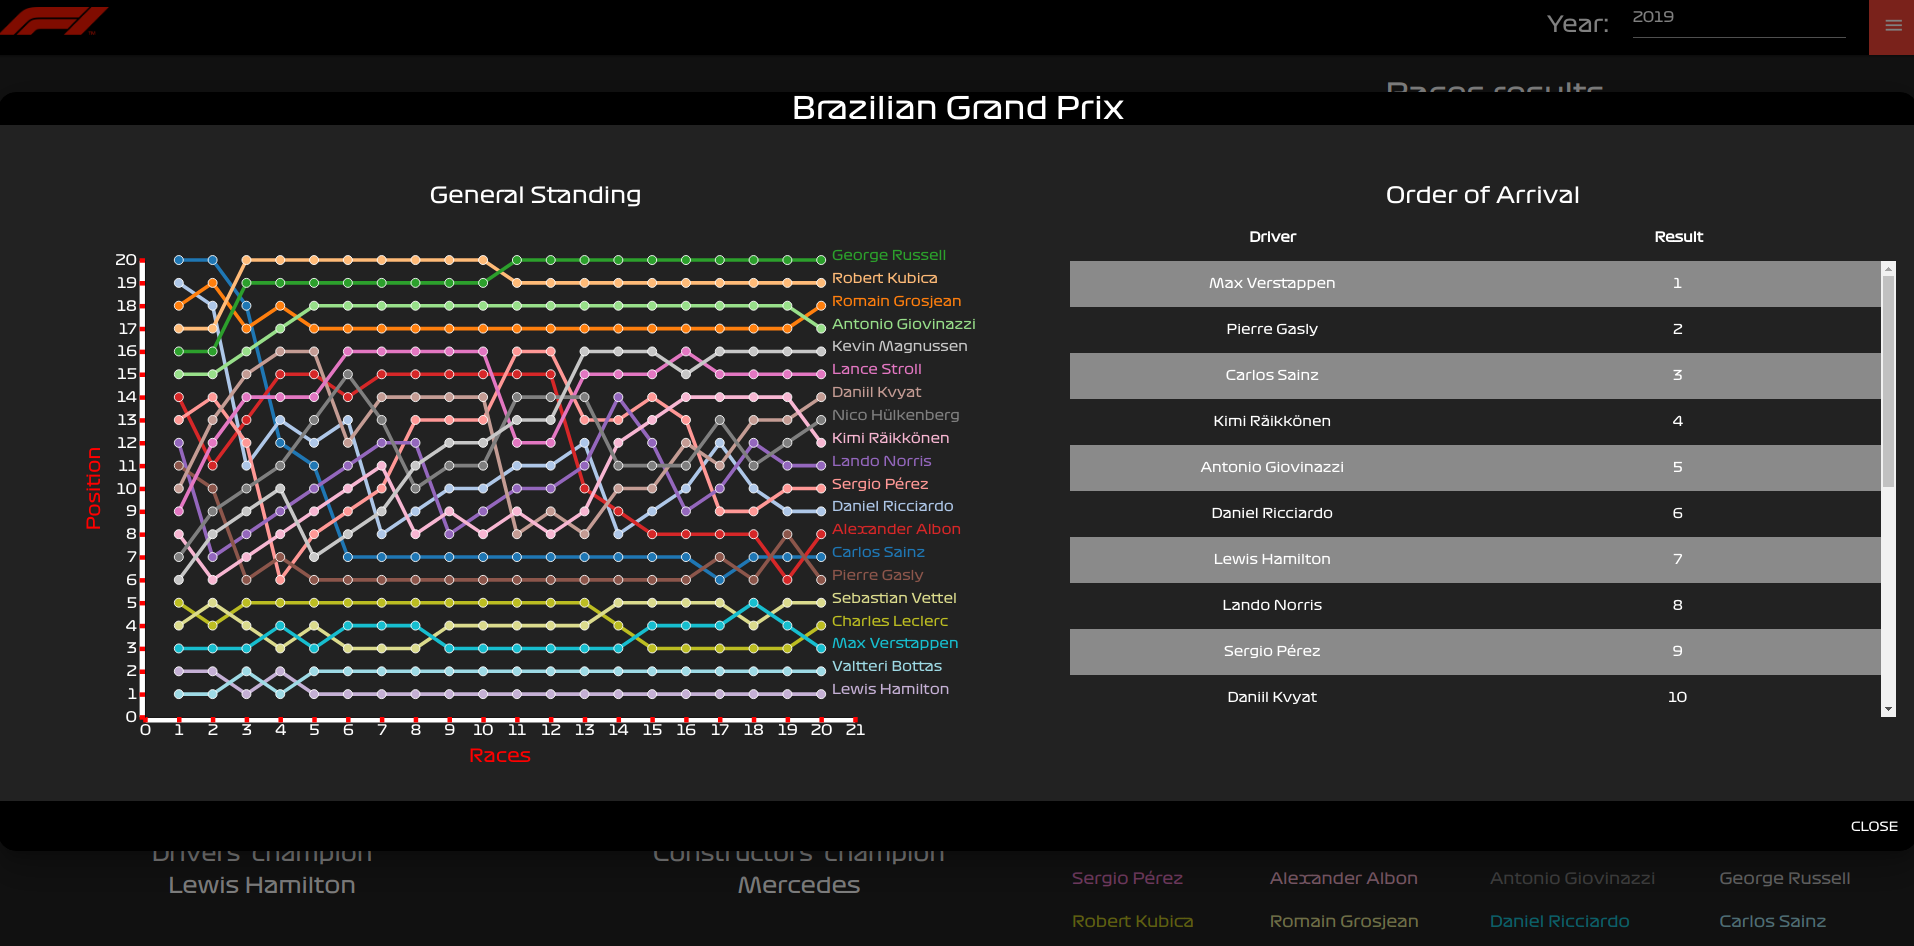
\includegraphics[width=\columnwidth]{map-clicked}
	\captionof{figure}{Home view}
\end{center}

\subsection{General info view}
\begin{center}
	\centering
	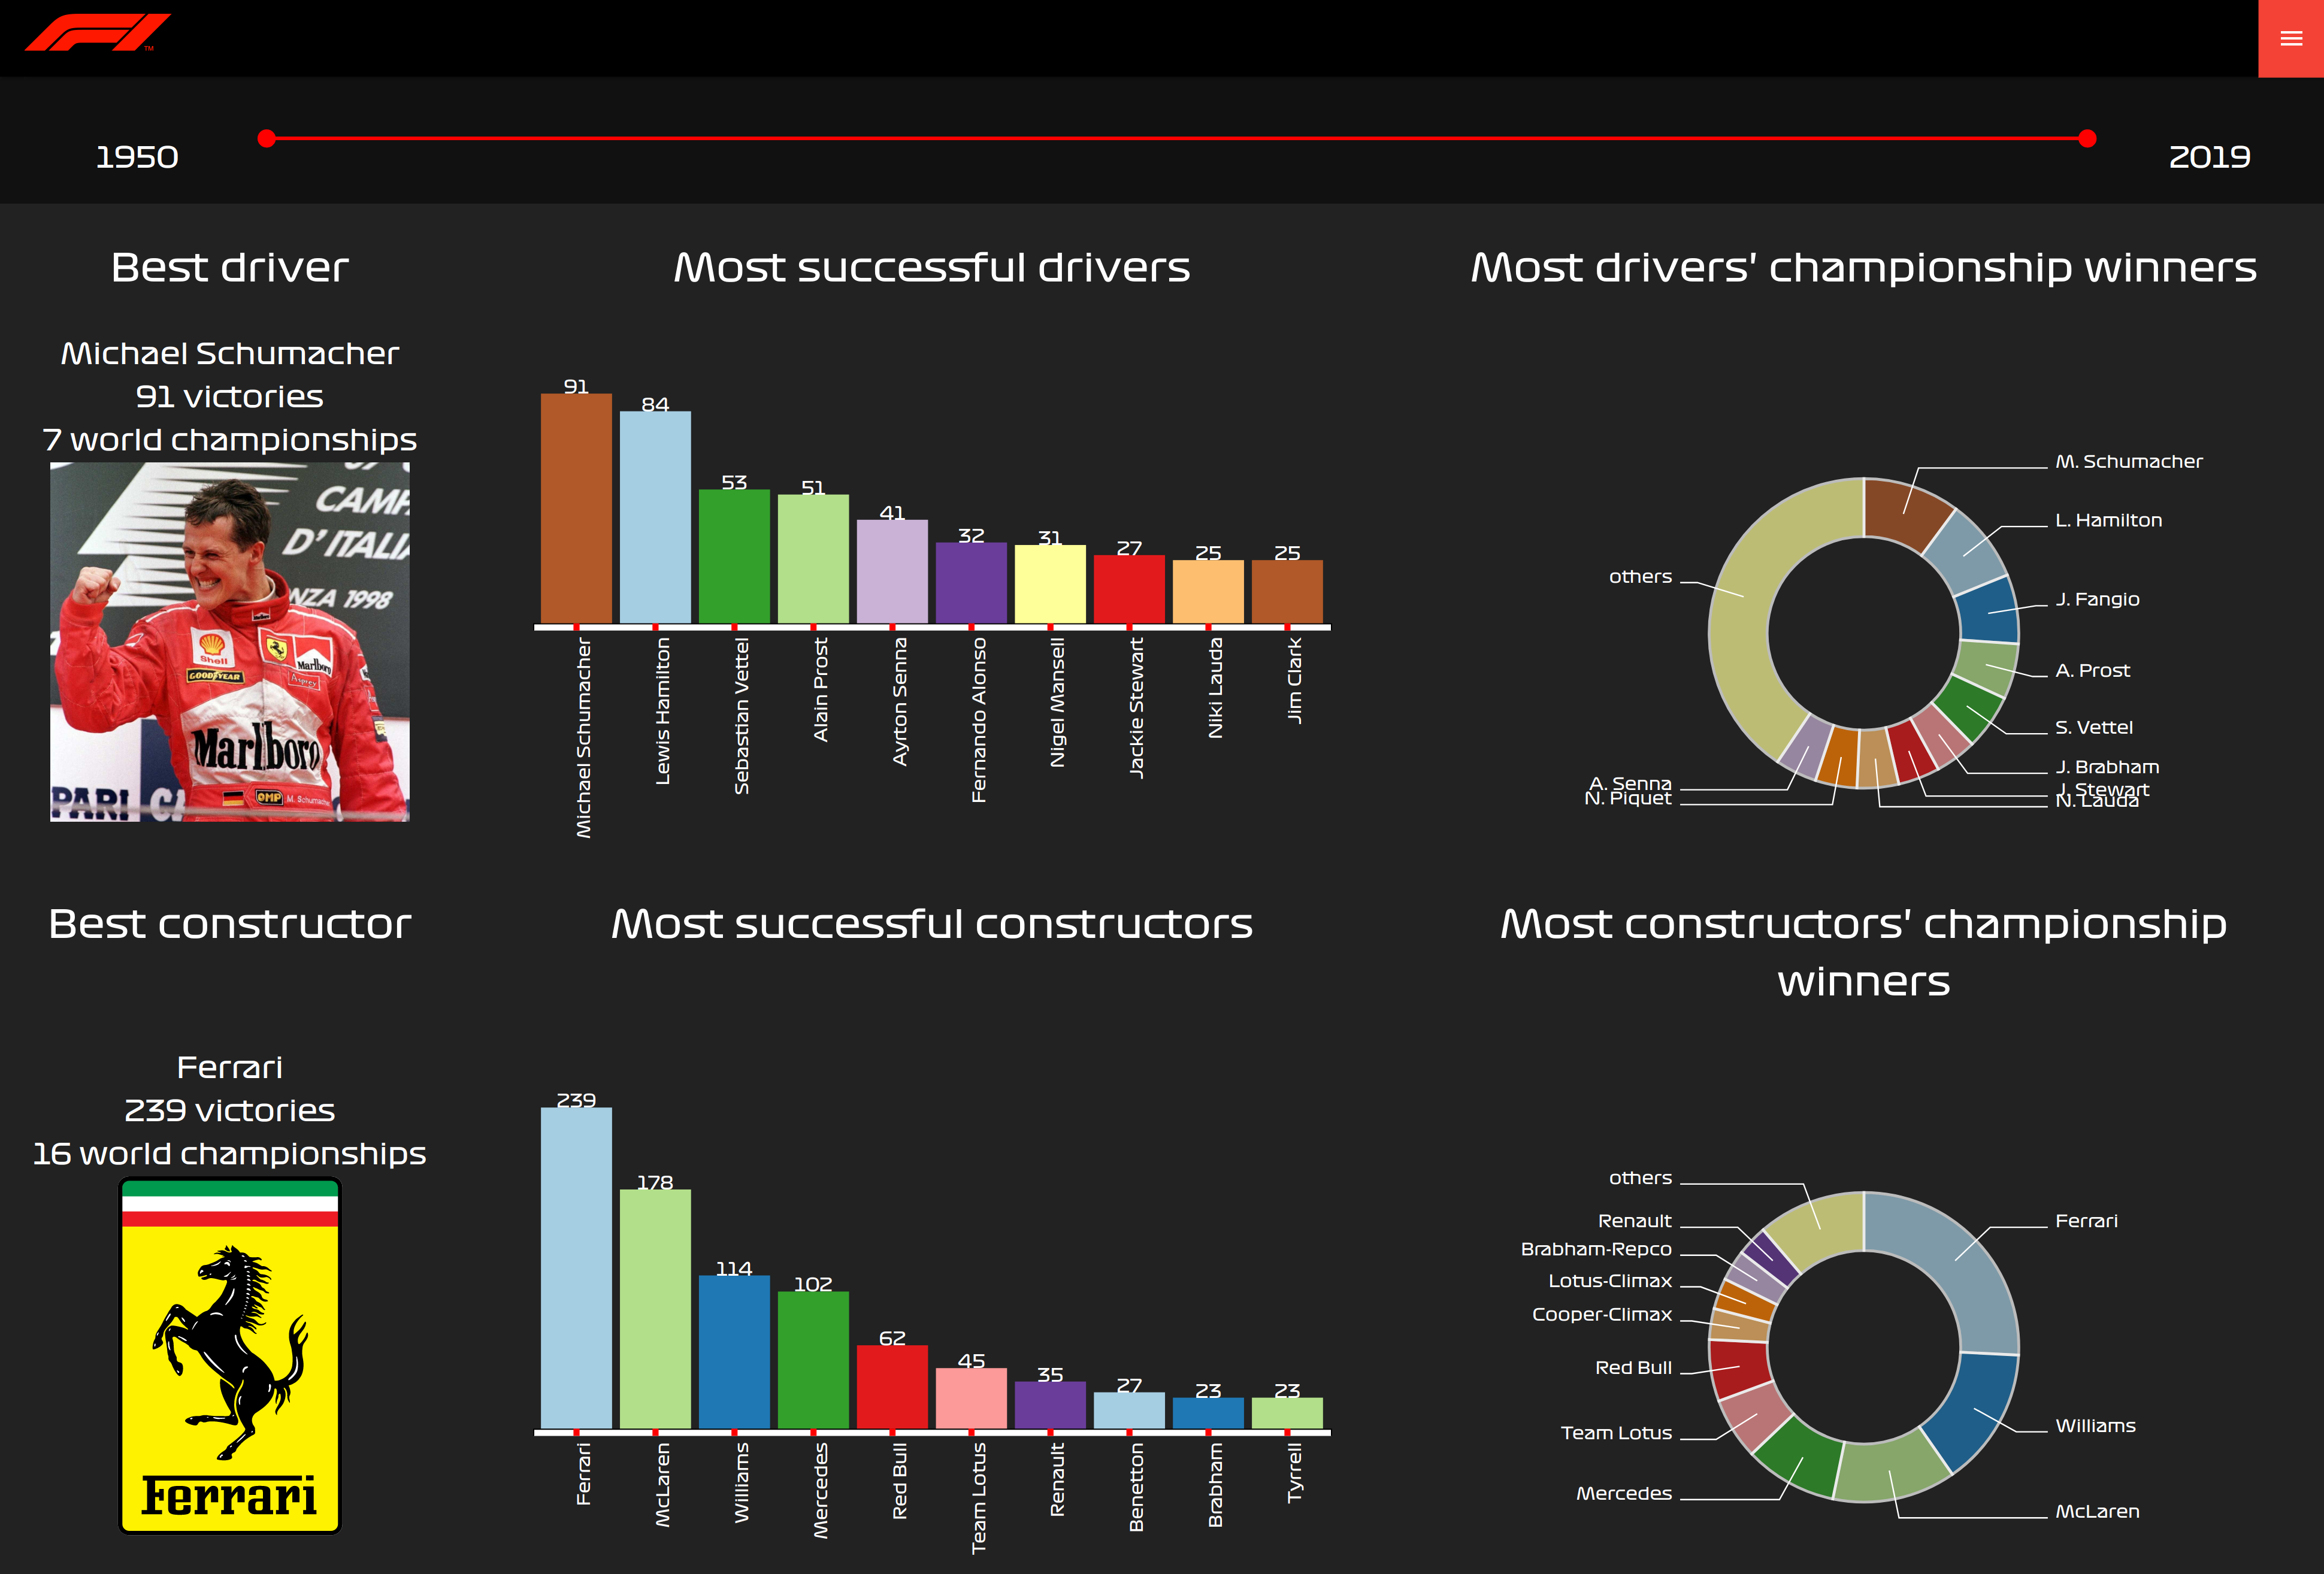
\includegraphics[width=\columnwidth]{generalinfo}
	\captionof{figure}{General info view}
\end{center}

\subsection{Correlations view}
\begin{center}
	\centering
	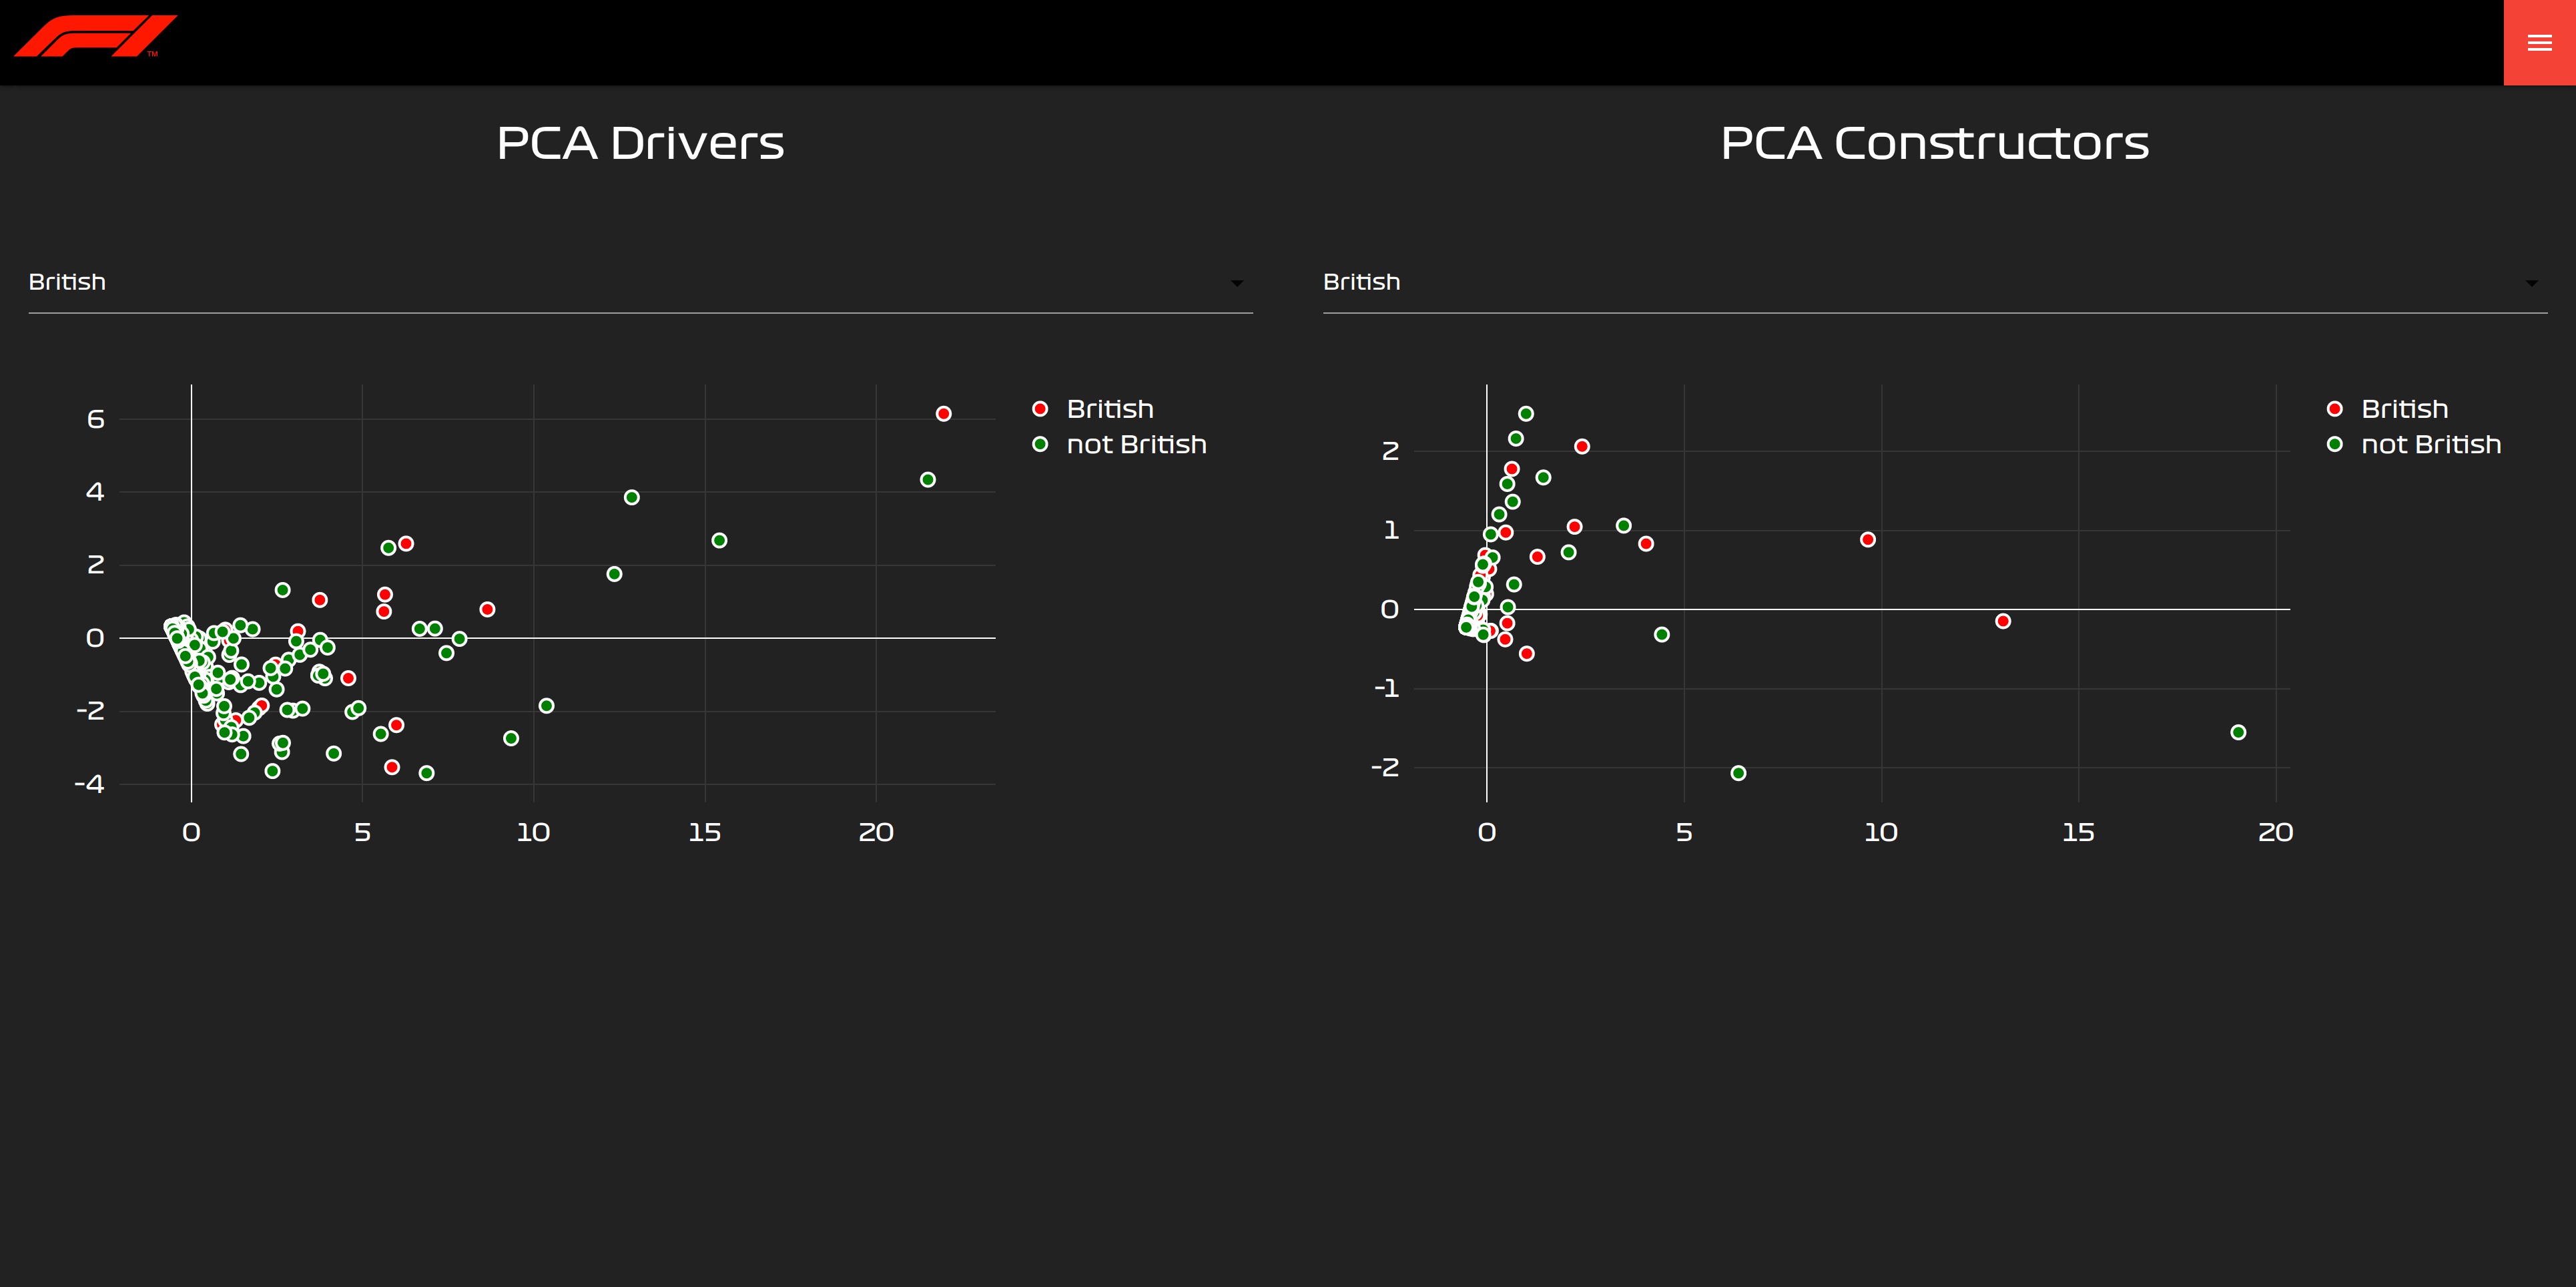
\includegraphics[width=\columnwidth]{correlations}
	\captionof{figure}{Correlations view}
\end{center}

\subsection{Times update view}
\begin{center}
	\centering
	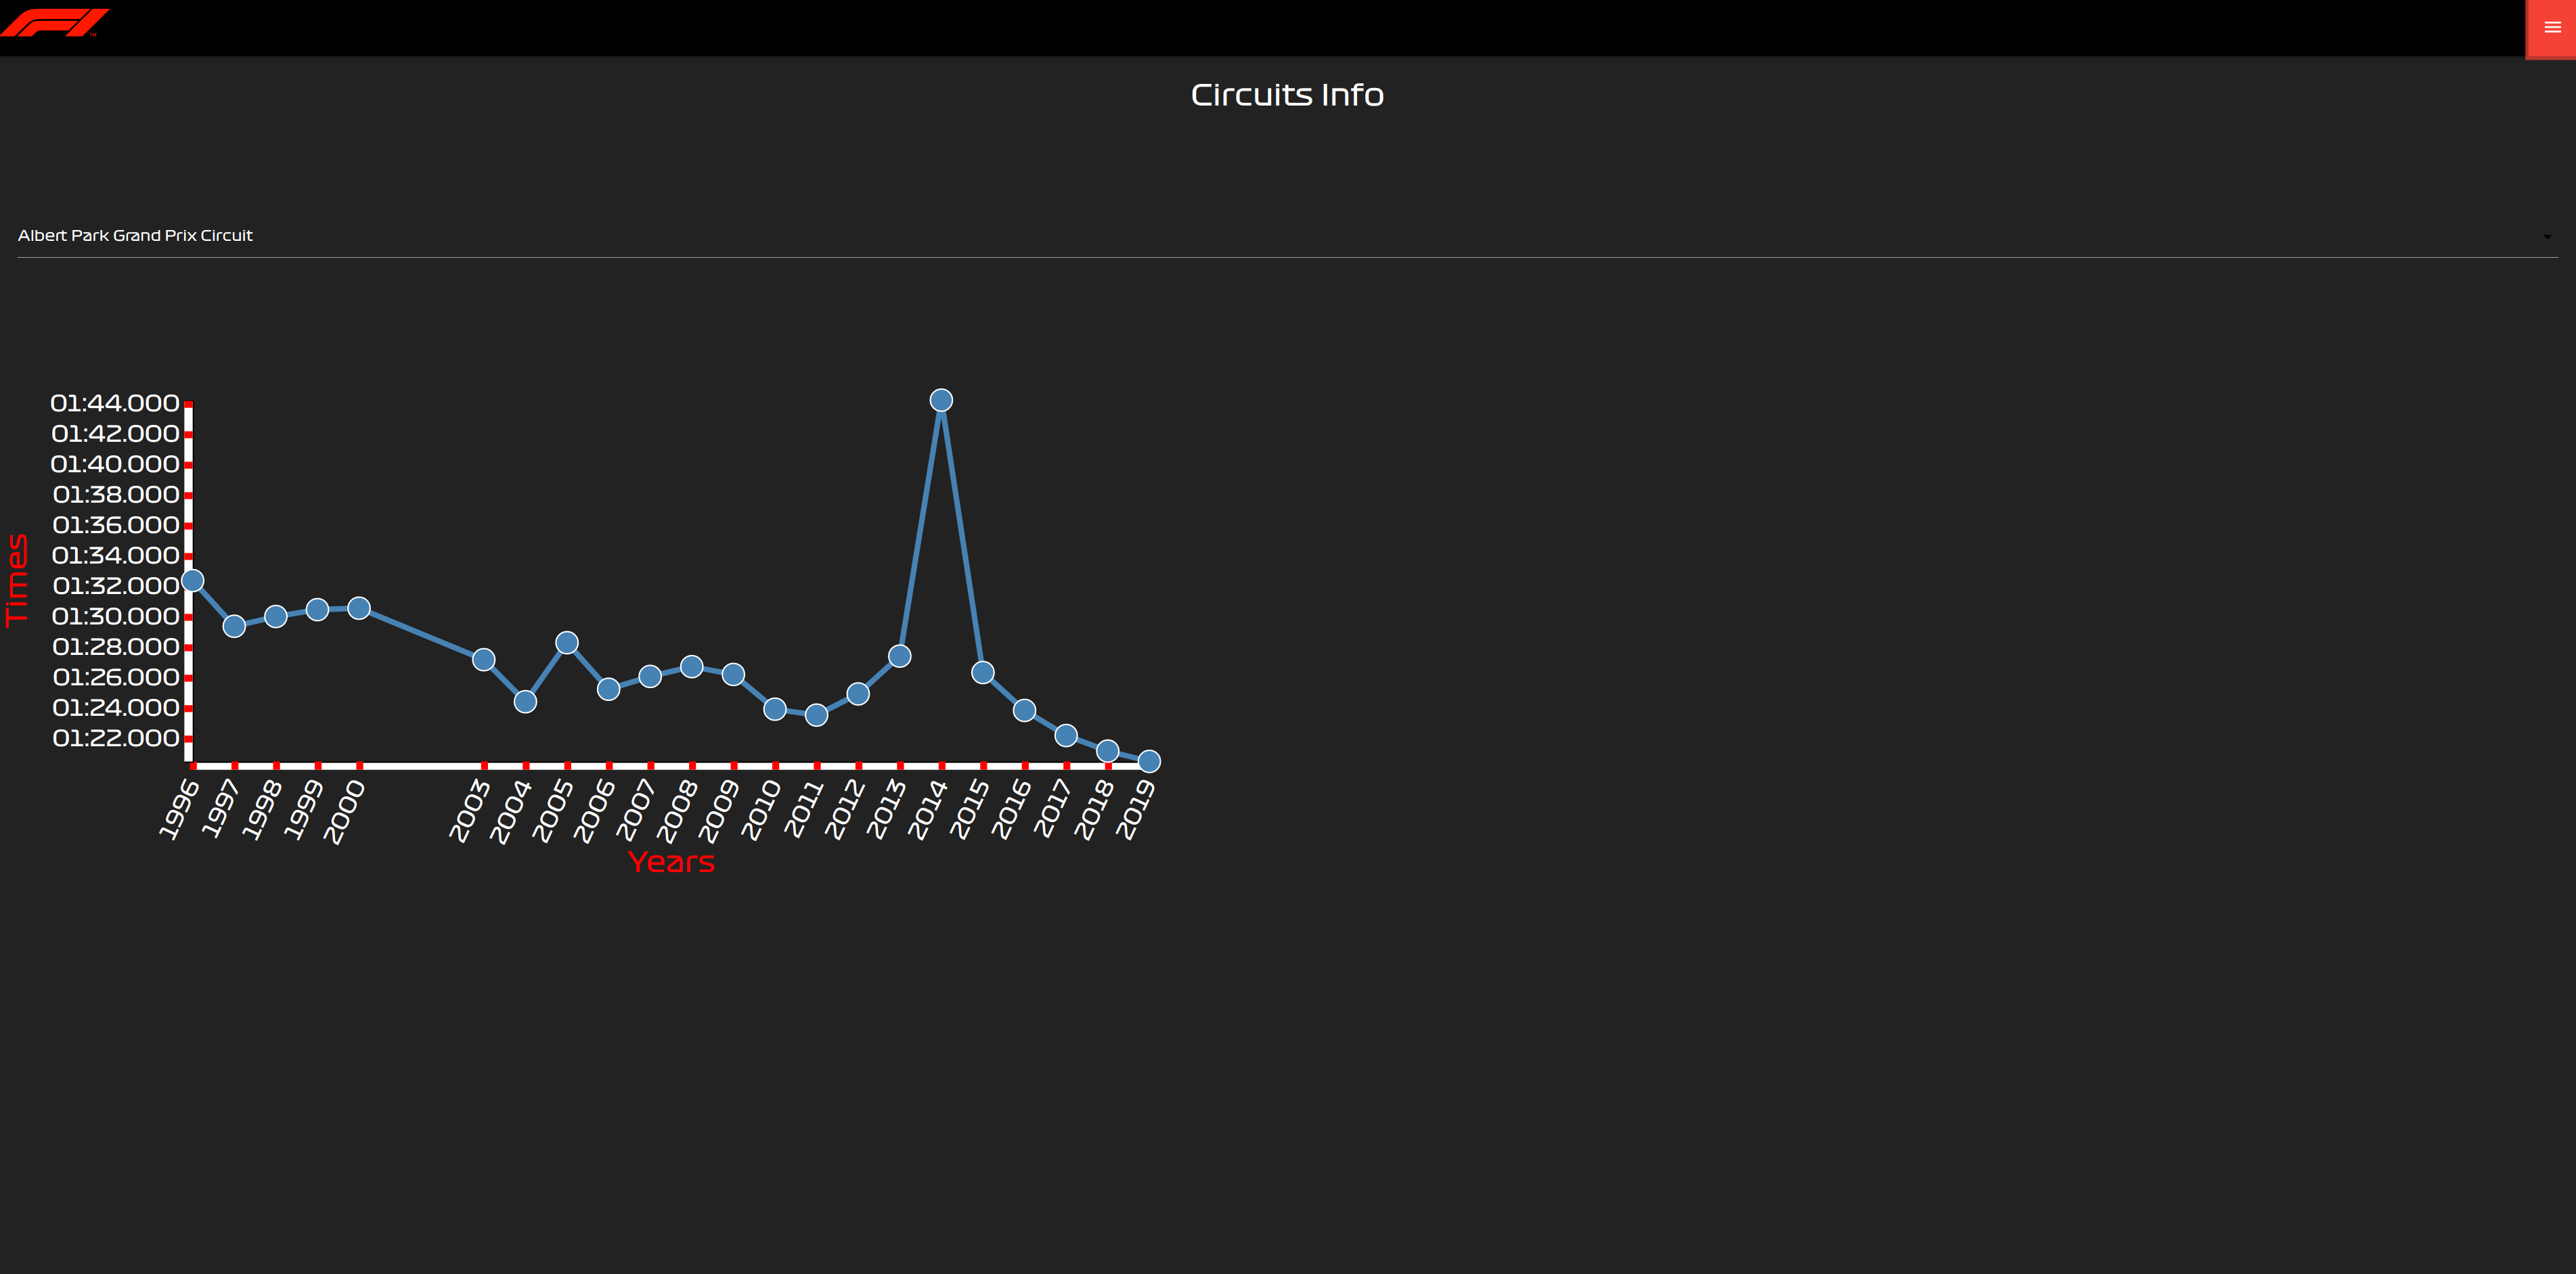
\includegraphics[width=\columnwidth]{timesupdate}
	\captionof{figure}{Times update view}
\end{center}


\section{Analytics}


\section{Future Works}

\section{Conclusion}
Conclusion text

\begin{thebibliography}{100} 
	\bibitem{D3} Data-Driven Documents: \href{https://d3js.org/}{https://d3js.org/}
	
	\bibitem{Dataset} Ergast Developer API: \href{http://ergast.com/mrd/}{http://ergast.com/mrd/}
	
	\bibitem{Plotly} Plotly JavaScript Open Source Graphing Library: \href{https://plot.ly/javascript/}{https://plot.ly/javascript/}
\end{thebibliography}

\end{document}
